\chapter{Patrones GoF}

\section{Introducción}

Estos 23 patrones de diseño son los patrones más conocidos y usados en la actualidad en el campo del Diseño Orientado a Objetos. \newline
En el año 1994, que apareció el libro “Design Patterns: Elements of Reusable Object Oriented Sofware” escrito por los ahora famosos Gang of Four (GoF, que en español es la pandilla de los cuatro) formada por Erich Gamma, Richard Helm, Ralph Johnson y John Vlissides. Los integrantes de la pandilla de los cuatro recopilaron y documentaron 23 patrones de diseño aplicados usualmente por expertos diseñadores de software orientado a objetos. Desde luego que ellos no son los inventores ni los únicos involucrados, pero ese fue luego de la publicación de ese libro que empezó a difundirse con más fuerza la idea de patrones de diseño. \newline
Los patrones de diseño el grupo de GoF clasifican en 3 grandes categorías basadas en su propósito: creacionales, estructurales y de comportamiento. \cite{gof}

“Los patrones de diseño son el esqueleto de las soluciones a problemas comunes en el desarrollo de software.”, es decir,  los patrones de diseño brindan una solución ya probada y documentada a problemas de desarrollo de software que están sujetos a contextos similares. 
Cuando se habla de un patrón de diseño es necesario tener presente los siguientes elementos que lo conforman: 
\begin{itemize}
	\item Nombre
	\item Problema: Define cuando se debe aplicar el patrón.
	\item Solución: Descripción abstracta de la respuesta que soluciona el problema.
	\item Consecuencias: Beneficios y costos de hacer el uso del patrón.
\end{itemize}  


Los patrones se pueden clasificar en tres categorías como se muestra a continuación:

\begin{itemize}
	\item Patrones Creacionales: Instanciación de objetos.
	\item Patrones Estructurales: Separan la interfaz de la implementación.
	\item Patrones de Comportamiento: Caracterizan las formas en  	las que interactúan y reparten responsabilidades las distintas clases u objetos.
\end{itemize}
\newpage




\section{Patrones Creacionales}
\paragraph{Definición}
Los patrones de diseño creacionales proporcionan ayuda a la hora de crear objetos apoyando el proceso de la toma de decisiones, incluso cuando esta toma de decisiones sea de forma dinámica. Además que tratan con las formas de crear instancias de objetos. El objetivo de estos patrones es de abstraer el proceso de instanciación y ocultar los detalles de cómo los objetos son creados o inicializados.
\paragraph{Tipos de Patrones}
Los patrones que se encuentran en la lista de Patrones Creacionales en el enfoque GOF son:
\begin{enumerate}
	\item Abstract Factory (Fábrica Abstracta)
	\item Factory Method (Método Fabrica)
	\item Prototype (Prototipo)
	\item Builder (Constructor)
	\item Singleton (Instancia Única)
\end{enumerate}


\subsection{Fabrica Abstracta}
\subsubsection{Modelo}
\newpage
\subsubsection{Caso}

	\begin{figure}[h!]
		\centering
		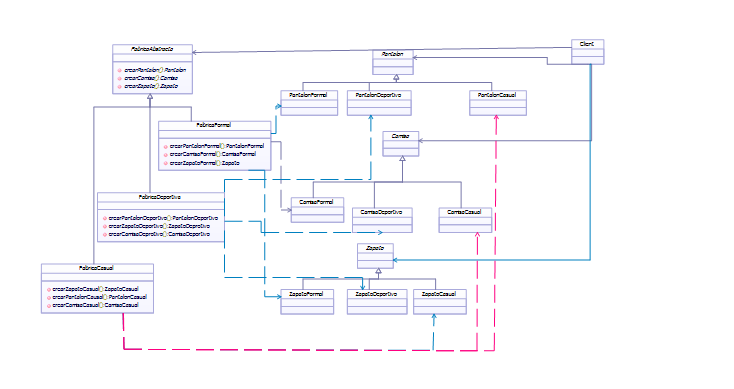
\includegraphics[width=1.2\linewidth]{arquitectura/imagenes/DiagramaFabricaAbstracta}
		\caption{Diagrama de clases Fabrica Abstracta}
	\end{figure}
	
	
	
	En el diagrama podemos ver que, para nuestro caso tendremos diferentes líneas de productos que podrán ser registrados en la base de datos. Para esto usamos el patrón fabrica abstracta que nos permite crear familias de productos de acuerdo a la línea establecida, además este patrón permite el escalamiento del aplicativo en forma horizontal, con lo cual, podremos a futuro adicionar otras nuevas líneas o colecciones de productos, sin necesidad de modificar las líneas ya creadas.
\newpage


\subsection{constructor}
\subsubsection{Modelo}
\newpage
\subsubsection{Caso}
\newpage

\subsection{Método Fábrica}
\subsubsection{Modelo}
\newpage
\subsubsection{Caso}
\newpage

\subsection{Prototipo}
\subsubsection{Modelo}
\newpage
\subsubsection{Caso}
\newpage

\section{Patrones Estructurales}
\paragraph{Definición}
Los patrones estructurales se enfocan en como las clases y objetos se componen para formar estructuras mayores, ademas describen como las estructuras compuestas por clases crecen para crear nuevas funcionalidades de manera que se puede agregar a la estructura flexibilidad y que la misma pueda cambiar en tiempo de ejecución lo cual es imposible con una composición de clases estáticas.
\paragraph{Tipos de Patrones}
Los patrones que se encuentran en la lista de Patrones Estructurales en el enfoque GOF son:
\begin{enumerate}
	\item Bridge (Puente)
	\item Adapter (Adaptador)
	\item Composite (Componente)
	\item Decorator (Decorador)
	\item Facade (Fachada)
	\item Flyweight (Peso Ligero) 
	\item Proxy (Proxy)
\end{enumerate}

\subsection{Adaptador}
\subsubsection{Modelo}
\newpage
\subsubsection{Caso}
\newpage


\subsection{Puente}\begin{figure}[h!]
	
\subsubsection{Modelo}
\newpage
\subsubsection{Caso}
\centering
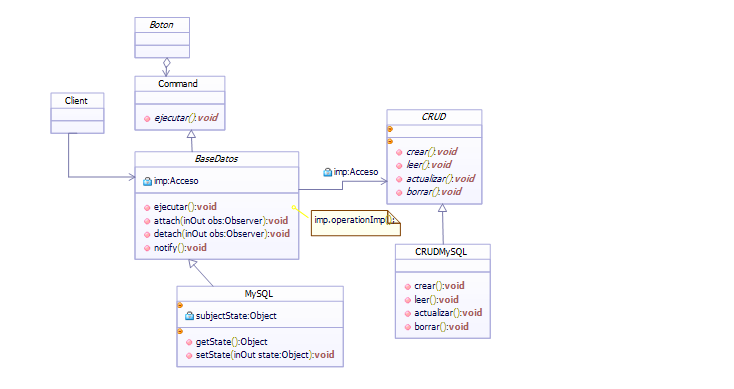
\includegraphics[width=1.0\linewidth]{arquitectura/imagenes/DiagramaComandoYPuente}
\caption{Diagrama de clases  Comando y Puente}
\end{figure}



El patrón comando utilizado en este caso permite separar y simplificar el uso de los botones y la función de cada uno en distintas opciones presentadas al usuario, para este caso particular están definidos los casos en los que el Admin crea, modifica, elimina o agrega un nuevo producto a la base de datos.
El patrón bridge, es un puente entre la abstracción de una base de datos y sus funciones con la lógica de estas funciones de acuerdo con el tipo de base de datos, puesto que la manera en que se borra, crea, agrega o modifica es diferente en cada base de datos (MySQL, Postgres, etc), de manera que en la base concreta se define el método en que cada función de la abstracción, realiza su operación. Esto permite que más adelante podamos agregar otras bases de datos a nuestro aplicativo sin la necesidad de modificar el código ya creado, y haciendo escalamiento de nuestro programa de manera horizontal.

\newpage

\subsection{componente}
\subsubsection{Modelo}
\newpage
\subsubsection{Caso}
\newpage

\subsection{Decorador}
\subsubsection{Modelo}
\newpage
\subsubsection{Caso}
\newpage

\subsection{Peso Ligero}
\subsubsection{Modelo}
\newpage
\subsubsection{Caso}
\newpage

\subsection{Proxy}
\subsubsection{Modelo}
\newpage
\subsubsection{Caso}
\newpage

\subsection{Fachada}
\subsubsection{Modelo}
\newpage
\subsubsection{Caso}
\newpage

\section{Patrones de Comportamiento}
\paragraph{Definición}
Los patrones de Comportamiento son los patrones ofrecen soluciones con respecto a la interacción y responsabilidades que hay entre objetos y clases, y las interacciones que hay entre estos ademas de los algoritmos que estos contiene.
\paragraph{Tipos de Patrones}
Los patrones que se encuentran en la lista de Patrones de Comportamiento en el enfoque GOF son:
\begin{enumerate}
	\item Command (Comando)
	\item Chain of Responsability (Cadena de responsabilidades)
	\item Iterator (Iterador)
	\item Interpreter (Interprete)
	\item Mediator (Mediador)
	\item Observer (Observador)
	\item State (Estado)
	\item Strategy (Estrategia)
	\item Template Method (Método Plantilla)
	\item Visitor (Visitante)
\end{enumerate}

\subsection{Comando}
\subsubsection{Modelo}
\newpage
\subsubsection{Caso}
\newpage

\subsection{Cadena de Responsabilidades}
\subsubsection{Modelo}
\newpage
\subsubsection{Caso}
\newpage

\subsection{Iterador}
\subsubsection{Modelo}
\newpage
\subsubsection{Caso}
\newpage

\subsection{Inrterprete}
\subsubsection{Modelo}
\newpage
\subsubsection{Caso}
\newpage

\subsection{Mediador}

\subsubsection{Modelo}
El patrón \textbf{Mediator o Mediador} define un objeto que hace de procesador central, y que se encarga coordinar las relaciones entre sus asociados o participantes. Este patrón permite la interacción de varios objetos, sin generar acoples fuertes en las relaciones. Todos los objetos se comunican con un mediador y es éste quién realiza la comunicación con el resto.
\begin{itemize}
	\item \textbf{Mediador: }Define una interface para comunicarse con los objetos colegas.
	\item \textbf{Mediador Concreto: }Implementa la interface y define como los colegas se comunican entre ellos.
	\item \textbf{Colega: }Define el comportamiento que debe implementar cada colega para poder comunicarse el mediador de una manera estandarizada para todos.
	\item \textbf{Colega Concreto: }Cada colega conoce su mediador, y lo usa para comunicarse con otros colegas.
\end{itemize}

%%\newpage
\subsubsection{Caso de estudio}

\begin{figure}[th!]
	\centering
	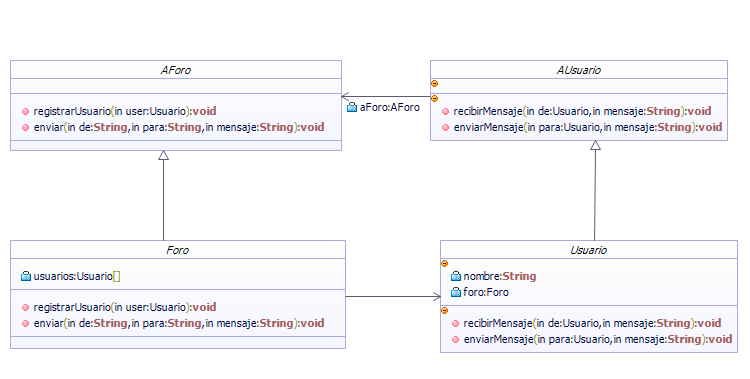
\includegraphics[width=1\linewidth]{arquitectura/imagenes/DiagramaMediator}
	\caption{Diagrama de clases Mediador}
\end{figure}

Para este caso en especifico se hace uso de patrón observador en su ejemplo más común no por simplicidad sino porque haciendo uso de este se satisface perfectamente uno de los principales requerimientos del sistema el cual es brindar un mecanismo para que a pesar de ser una tienda virtual los usuarios puedan seguir comunicandose con los asesores. \newline
En este caso se plantea una interfaz abstracta para cada usuario que tiene dos métodos, enviar y recibir mensaje, esta se implementa en cada usuario que a su vez tiene un nombre que lo identifica en el foro y le permitirá distinguirse de los demás y ademas conoce el foro. La interfaz abstracta AForo tiene dos métodos que permiten a los usuarios suscribirse al foro y el método enviar que es donde se realizara todo el proceso de registro y envio del mensaje, esta interfaz la implementa la Clase Foro que además tiene un arreglo de usuarios que son los usuarios que pertenecen al chat.

\newpage

\subsection{Momento}
\subsubsection{Modelo}
\newpage
\subsubsection{Caso}
\newpage

\subsection{Observador}
\subsubsection{Modelo}
\newpage
\subsubsection{Caso}
	\begin{figure}[h!]
	\centering
	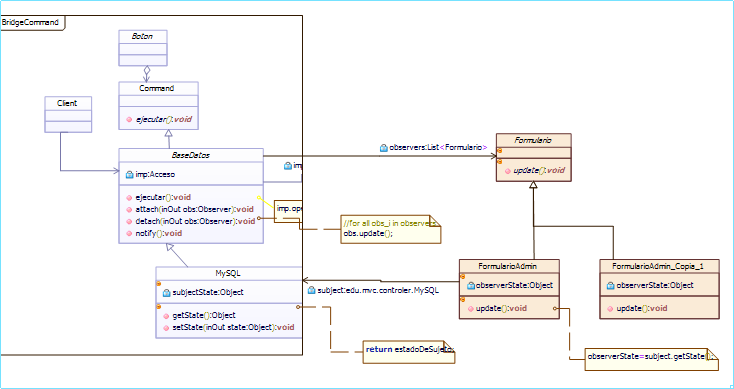
\includegraphics[width=1.0\linewidth]{arquitectura/imagenes/DiagramaObservador}
	\caption{Diagrama de clases patrón Observador}
\end{figure}



El patrón observador es utilizado en nuestro caso debido a la necesidad que tenemos de estar actualizando constantemente los datos de los productos en los formularios del Admin y el Cliente, ya sea actualizando el estado del producto en el stack, o alguna de sus características cada vez que entramos a modificarlas, este patrón nos permite facilitar esta actualización directamente en nuestra base de datos
\newpage

\newpage

\subsection{Estado}
\subsubsection{Modelo}
\newpage
\subsubsection{Caso}
\newpage

\subsection{Estrategia}
\subsubsection{Modelo}
\newpage
\subsubsection{Caso}
\newpage

\subsection{Visitador}
\subsubsection{Modelo}
\newpage
\subsubsection{Caso}
\newpage

\subsection{Método Plantilla}
\subsubsection{Modelo}
\newpage
\subsubsection{Caso}
\begin{figure}[h!]
	\centering
	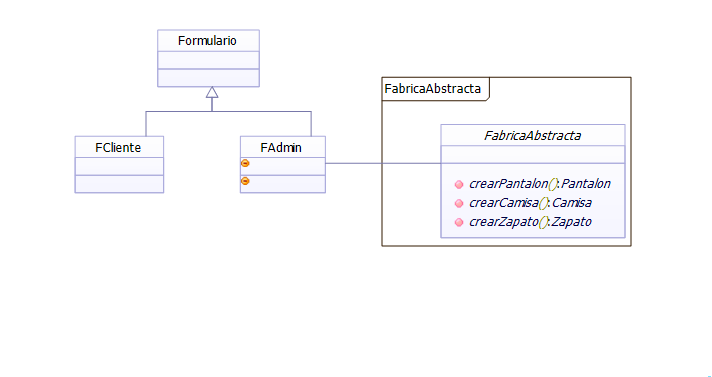
\includegraphics[width=1.0\linewidth]{arquitectura/imagenes/DiagramaFachada}
	\caption{Diagrama de clases patrón Fachada}
\end{figure}



Este patrón nos permite ocultar al cliente y al admin lo que sucede detrás del formulario que utilizan, es decir oculta la lógica del programa, la cual no es interesante para ellos, podemos incluir varios subsistemas con este patrón y dejarlos solo visibles para los realmente interesados en cada uno.

\newpage